\documentclass[11pt]{article}

\usepackage{graphicx}
\usepackage{amsmath}
\usepackage{siunitx}
\usepackage[a4paper, total={6in, 10in}]{geometry}
\usepackage{titling}
\usepackage{listings}
\usepackage{float}
\usepackage{subcaption}
\usepackage{pdfpages}
\usepackage{bbm}


\newcommand{\Lik}{\mathcal{L}}

\graphicspath{{figures/}}
\title{\vspace{-2cm}4F13 Coursework 2 - Probabilistic Ranking}
\preauthor{}
\author{}
\postauthor{}
\date{November 2024}

\begin{document}

% 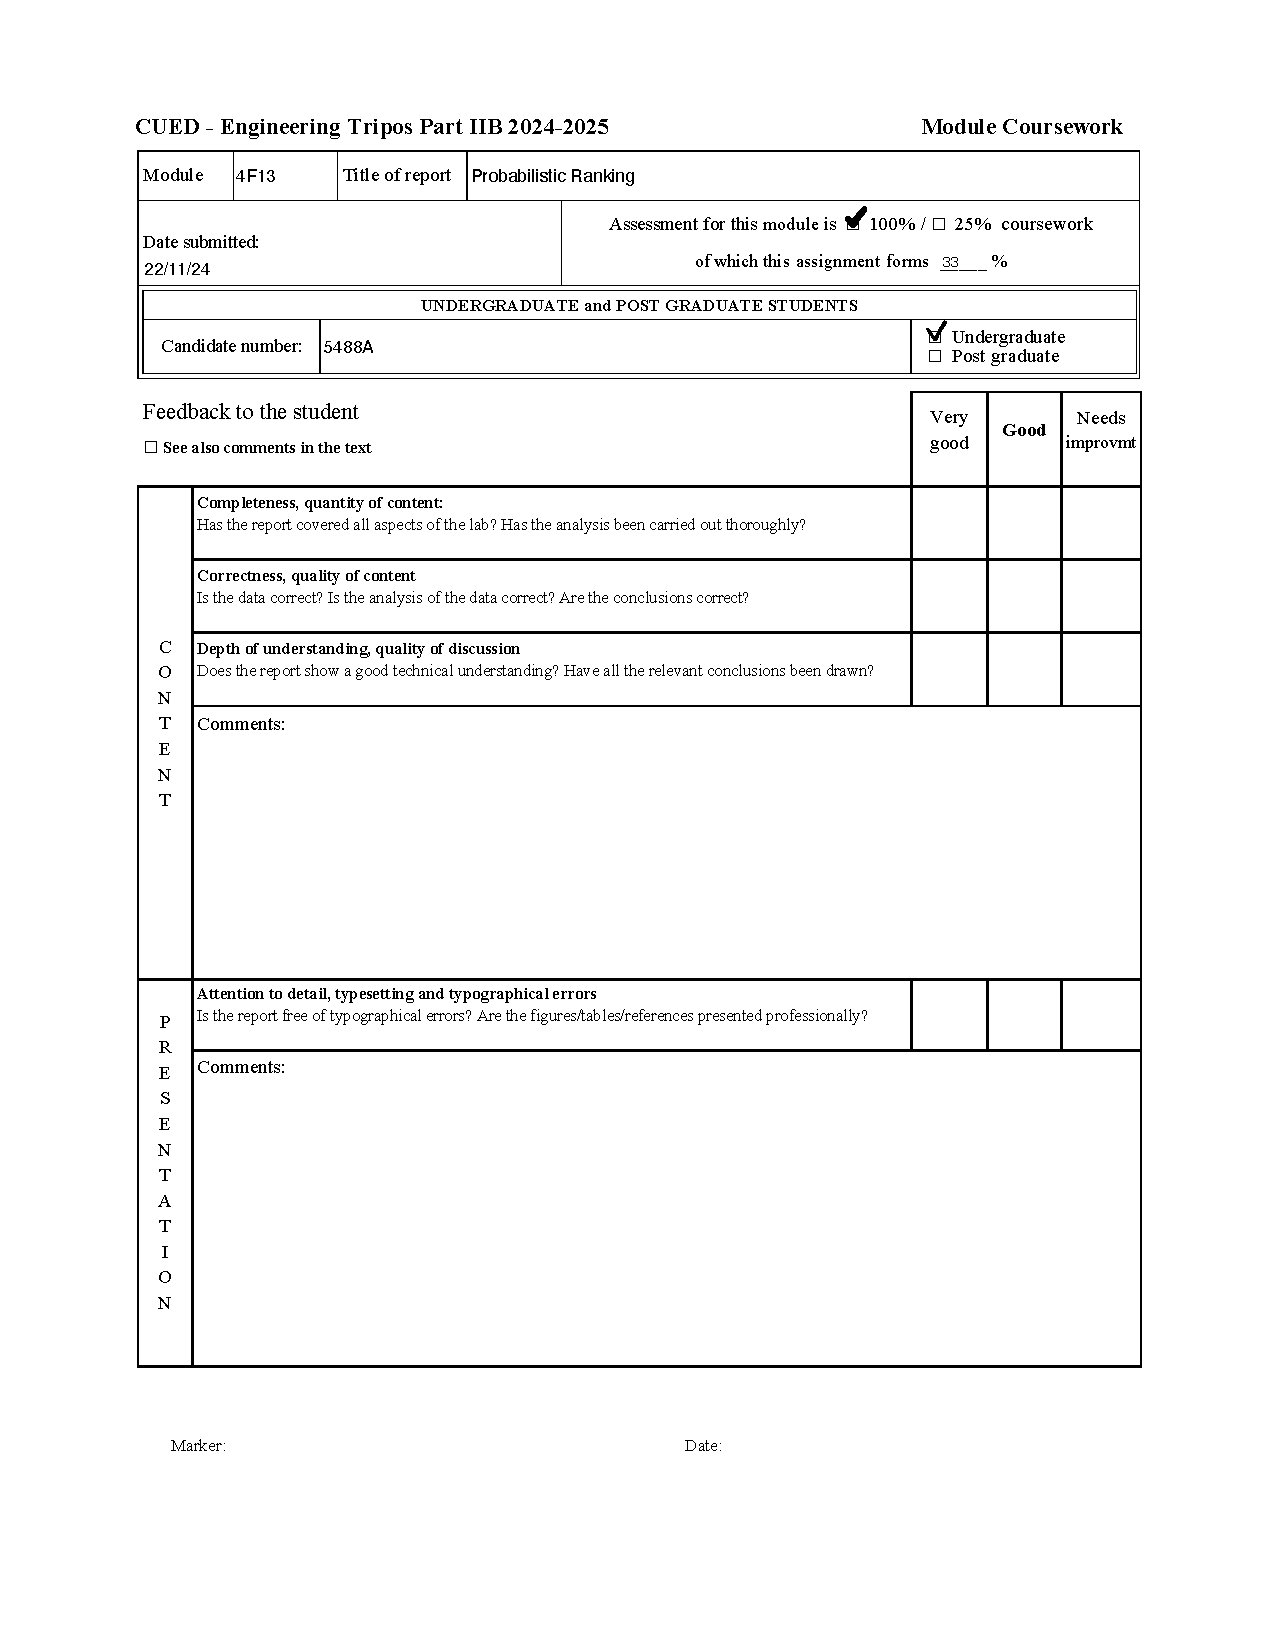
\includepdf[pages={1}]{coversheet}

\setcounter{page}{1}

\maketitle

\section{Task A}

Figure \ref{fig:A_skill_samples} shows samples of the skills at each Gibbs iteration for 3 players. We see that at each iteration the skill of each player appears random but perhaps not independent of the previous iteration. This is as expected from Gibbs sampling and is demonstrated by the auto covariance plot in Figure \ref{fig:A_auto_covariance}. 

\begin{figure}[h]
    \centering
    \includegraphics[width=\linewidth]{A/skill_samples} 
    \caption{Samples of the skill of 3 players at each Gibbs iteration.}
    \label{fig:A_skill_samples}
\end{figure}

If the samples at each iteration were independent we would expect the auto covariance to be zero for all non zero lags. However, we notice that the auto covariance only converges to zero for lags greater than about 5. This indicates that if we kept only every 5th sample they would be independent, this is the logic behind thinning. We are not running into computational/memory limits in this case so there is no need to thin the samples.

\begin{figure}[h]
    \centering
    \includegraphics[width=\linewidth]{A/auto_covariance} 
    \caption{Auto covariance of the skill of all players}
    \label{fig:A_auto_covariance}
\end{figure}

The convergence of the skill population is shown in Figure \ref{fig:A_convergence}. We see that there is no clear burn in time for the population mean but the standard deviation needs about 5 iterations to converge. This makes sense from our auto covariance analysis as we concluded samples 5 iterations apart are roughly independent. For any further we will discard the first 5 Gibbs iterations as burn in time.

\begin{figure}[h]
    \centering
    \includegraphics[width=\linewidth]{A/convergence} 
    \caption{Skill populations mean and standard deviation with Gibbs iteration.}
    \label{fig:A_convergence}
\end{figure}

To estimate how many iterations we need to run the Gibbs sampler to get skill estimates within a certain tolerance we can analyse the variance of our Monte Carlo skill estimates. Equation \ref{eq:gibbs_skill_variance} calculates the variance of the estimated skill of player $i$ after $M$ Gibbs iterations, the first two equalities are the standard Monte Carlo variance result with $N$ independent samples $w_i^{(n)}$. The final approximate equality is by setting $M=5N$ as we found that samples are roughly independent every 5 Gibbs iterations.

\begin{equation}
    \text{Var}(\bar{w_i}) = \text{Var}(\frac{1}{N} \sum_{n=1}^{N} w_i^{(n)})  = \frac{1}{N} \text{Var}(w_i) \approx \frac{5}{M} \text{Var}(w_i)
    \label{eq:gibbs_skill_variance}
\end{equation}
We take this result and compute the number of Gibbs iterations required to have 95\% confidence that the skill estimate is within 1\% of the true skill in Equation \ref{eq:gibbs_iterations}. Here we assume that the marginal skill mean, $\mu_{w_i}$, is of order $1$ due to our prior variance. This gives a result of $M \approx 1\times10^4$ iterations where we use the median $Var(w_i)$.
\begin{equation}
    \frac{2*\sqrt{\text{Var}(\bar{w_i})}}{\mu_{w_i}} = 0.01 \implies M \approx 2\times10^5 \times \text{Var}(w_i)
    \label{eq:gibbs_iterations}
\end{equation}

\section{Task B}

In the previous section we saw that it took about 10000 iterations for the Gibbs sampled skill estimates to converge within our tolerance. In comparison, Figure \ref{fig:B_convergence} shows that the EP skill estimates converge within 10 iterations for the given players.

\begin{figure}[h]
    \centering
    \includegraphics[width=\linewidth]{B/convergence} 
    \caption{EP skill parameter evolution with iteration for 5 players.}
    \label{fig:B_convergence}
\end{figure}

\section{Task C}

Using the skill parameters estimated by the EP algorithm we denote the skill of player $i$ as $w_i \sim \mathcal{N}(m_i, p_i^{-1})$, with $m_i$ and $p_i$ being the mean and precision for player $i$. The distributions of the skill difference, $s_{ij} = w_i - w_j$, and performance difference, $t_{ij} = s_{ij} + \eta : \eta \sim \mathcal{N}(0, 1)$, between player $i$ and $j$ are given in Equation \ref{eq:skill_performance_diff}. These are simple to compute under the assumption that $w_i$, $w_j$ and $\eta$ are independent.

\begin{equation}
\begin{split}
    s_{ij} &\sim \mathcal{N}(m_i - m_j, p_i^{-1} + p_j^{-1}) \\
    t_{ij} &\sim \mathcal{N}(m_i - m_j, p_i^{-1} + p_j^{-1} + 1)
\end{split}
\label{eq:skill_performance_diff}
\end{equation}

We wish to compute the probability that player $i$ has greater skill that player $j$, $P(s_{ij}>0)$, and the probability that player $i$ will win a match against player $j$, $P(t_{ij}>0)$. We use the identity $P(x>0) = \phi(\frac{\mu}{\sigma})$ where $\phi$ is the standard normal c.d.f. and $x \sim \mathcal{N}(\mu, \sigma^2)$. We find these probabilities between the top 4 ranked ATP players in Table \ref{tbl:B_atp_probabilities}.

\begin{table}
    \centering
    \small
    \begin{minipage}{0.45\textwidth}
        \centering
        \begin{tabular}{|c|c c c c|}
            \hline
            $P(s_{ij}>0)$ & Djokovic & Nadal & Federer & Murray \\
            \hline
            Djokovic & -    & 0.94 & 0.91 & 0.99 \\
            Nadal    & 0.06 & -    & 0.43 & 0.77 \\
            Federer  & 0.09 & 0.57 & -    & 0.81 \\
            Murray   & 0.01 & 0.23 & 0.19 & -    \\
            \hline
        \end{tabular}
        \subcaption{Probability that row player is more skilled that column player.}
        \label{tbl:B_skill_difference}
    \end{minipage}
    \begin{minipage}{0.45\textwidth}
        \centering
        \begin{tabular}{|c|c c c c|}
            \hline
            $P(t_{ij}>0)$ & Djokovic & Nadal & Federer & Murray \\
            \hline
            Djokovic & -    & 0.94 & 0.91 & 0.99 \\
            Nadal    & 0.06 & -    & 0.43 & 0.77 \\
            Federer  & 0.09 & 0.57 & -    & 0.81 \\
            Murray   & 0.01 & 0.23 & 0.19 & -    \\
            \hline
        \end{tabular}
        \subcaption{Probability that row player wins a match against column player.}
        \label{tbl:B_performance_difference}
    \end{minipage}
    \caption{Skill and performance differences between top 4 ATP players based on EP.}
    \label{tbl:B_atp_probabilities}
\end{table}

We are always more confident in who is more skilled that who will win a match. This makes sense as $\sigma_t > \sigma_s$, however, intuitively this is clear as we are always less certain about the outcome of a match due to performance variation.

\section{Task D}
Using our Gibbs samples we would like to estimate the skill difference between Nadal and Federer. We investigate three methods to do this in the following sections.

\subsection{Approximate marginal skills with gaussians}
We compute the samples mean and variance for each player and model their skills as $w_i \sim \mathcal{N}(\mu_i, \sigma_i^2)$. Figure \ref{fig:D_marginals} shows sample histograms and gaussian approximation. Using the formulas from Task C we find that $P(w_{Nadal} > w_{Federer}) = 0.395$.

\begin{figure}
    \centering
    \includegraphics[width=0.75\linewidth]{D/marginals}
    \caption{Marginal skill distributions and gaussian approximations for Nadal and Federer.}
    \label{fig:D_marginals}
\end{figure}

\subsection{Approximate joint skill distribution with a multivariate gaussian}
We can also approximate the joint skill distribution with a gaussian by computing the sample covariance matrix. We find a positive covariance between the two players, $\sigma_{ij}^2 = 0.01$. We visualise the joint distribution and our approximation in Figure \ref{fig:D_joint}.

\begin{figure}
    \centering
    \includegraphics[width=0.75\linewidth]{D/joint}
    \caption{Joint skill distribution (histogram) and gaussian approximation (contours) for Nadal and Federer.}
    \label{fig:D_joint}
\end{figure}

\subsection{Use the samples directly}
We can also compute a Monte Carlo estimate of $P(w_{Nadal} > w_{Federer})$. This estimate is given in Equation \ref{eq:D_monte_carlo} where $(w_{i}^{(n)}, w_{j}^{(n)})$ are samples from a Markov chain with stationary distribution $p(w_{i}, w_{j})$. Our Gibbs samples satisfy this condition and we find $P(w_{Nadal} > w_{Federer}) = 0.395$.

\begin{equation}
    \begin{split}
    \text{P}(w_{i} > w_{j}) &= \text{E}(\mathbbm{1}(w_{i} > w_{j})) \\
     &=  \int \mathbbm{1}(w_{i} > w_{j}) p(w_{i}, w_{j}) dw_{i} dw_{j} \\
     &\approx \frac{1}{N} \sum_{n=1}^{N} \mathbbm{1}(w_{i}^{(n)} > w_{j}^{(n)})
    \end{split}
    \label{eq:D_monte_carlo}
\end{equation}

\section{Task E}

We have explored methods for skill estimation using both Gibbs sampling and EP algorithms. A simpler model for estimating skill is to assume every player has a fixed win rate $r_i$. The posterior distribution of $r$ for a player who wins $k$ out of $n$ matches with a uniform prior is the Beta distribution given in Equation \ref{eq:E_win_rate_posterior}. We can apply the central limit theorem to approximate this posterior with a gaussian for large $n$. We interpret this win rate as the skill of the player and plot its mean and 66\% error bars in Figure \ref{fig:E_skill_estimates} along with those obtains from Gibbs sampling and EP.

\begin{equation}
    r|k,n \sim \text{Beta}(1+k, 1+n-k) \approx \mathcal{N}(\frac{k}{n}, \frac{k(n-k)}{n^3})
    \label{eq:E_win_rate_posterior}
\end{equation}

\end{document}